%   Filename    : chapter_4.tex 
\chapter{Results \& Discussions}
\section{Dataset}
We built a dataset containing a total of 1155 Gen Z internet slang sentences and their corresponding formal translations. The created dataset was then combined with another dataset from Hugging Face that contains 698 Gen Z internet slang and their corresponding formal translation.
 
\section{Model Evaluation}
\subsection{Model Training}
The model was trained for 7 epochs before the early stopping callback was triggered because the evaluation metrics has not improved by at least 0.01 for 3 consecutive epochs. This prevented the overfitting seen in the following figure. 
% {Insert Figure here}

Here, we can see that the while the training loss is decreasing, the validation loss is increasing and other metrics are not improving. This indicates that the model is overfitting to the training data and may not generalize well to new data. The model training was stopped in just 7 epochs and the best model amongst the epochs, the one with the lowest validation loss and highest metrics, was chosen as the final model.

\subsection{Text Generation}
A total of 197 sentences were translated using both the base zephyr-7b-beta model and the finetuned model. These served as the dataset used to evaluate the performance of the model and comparing it with the other base model.

\subsection{Automatic Evaluation Metrics}
The dataset was automatically evaluated using BLEU and ROUGE metrics, specifically the ROUGE-L metric as the dataset do not contain newlines that ROUGE-Lsum uses to separate the input with. These scores were then averaged to determine the score of the models. The base model obtained a BLEU score of 0.8099 and ROUGE-L Score of 0.8336 and the finetuned model obtained a BLEU score of 0.8151 and ROUGE-L Score of 0.8396. While the difference between the models is minimal, this does not completely represent the performance of the models as these metrics are only used to determine if the generated text is close to the reference text, regardless of the context and the overall quality of the generated text. However, it does show that the finetuned model, while not significantly better than the base model, is close to the reference model.

\begin{figure}
	\caption{Automatic Evaluation of Dataset using BLEU and ROUGE metrics.}
	\centering
	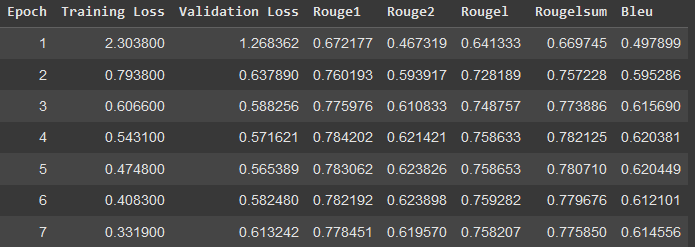
\includegraphics[scale=0.6]{figures/AutomaticEvaluationMetrics.png}
\end{figure}

\subsection{Manual Evaluation Metrics}
\section{Summary}

